\documentclass[border=10pt]{standalone}
\usepackage{tikz}
\begin{document}
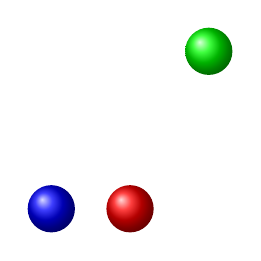
\begin{tikzpicture}
%\path[draw] (0, 0) -- (1, 1) -- (2, 0);
%\path[draw, line width=4pt] (1, 1) -- (2, 2) -- (3, 1) -- cycle;
%\path[draw, fill=green!50] (1, 1) -- (2, 2) -- (3, 1) -- cycle;
% \path[draw, fill=green] (1, 1) -- (2, 2) -- (3, 1) -- cycle;
% \path[clip, draw] (1, 1) -- (2, 2) -- (3, 1) -- cycle;
% \path[fill=blue!50] (2, 2) circle (1);
%\path[shade, draw] (1, 1) -- (2, 2) -- (3, 1) -- cycle;
% \path[shade, left color = blue] (1, 1) -- (2, 2) -- (3, 1) -- cycle;
% \path[shading = ball, ball color = blue] (1, 1) -- (2, 2) -- (3, 1) -- cycle;
\path[shading = ball, ball color = blue]  (0, 0) circle (0.3);
\path[shading = ball, ball color = red]   (1, 0) circle (0.3);
\path[shading = ball, ball color = green] (2, 2) circle (0.3);
\end{tikzpicture}
\end{document}